% !TeX encoding = UTF-8
% !TeX spellcheck = en_GB
\section{Monitoring}
\subsection{Prometheus}
\subsubsection{Decision Log}
\paragraph{} Prometheus is a powerful and widely used open-source tool for systems monitoring. We chose this tool for its open-souce nature, ease of use, powerful query language and simple interoperability with Grafana. Prometheus was used as a docker container running on our VMs and it was used for quering monitoring data about our running .NET minitwit application
\paragraph{} Setting up Prometheus really was as easy as just getting a docker image of it running. All the data source configuring was done through Grafana, including all visualization of the data itself. This ease of use was very evident and convenient.

\subsection{Grafana}
\subsubsection{Decision Log}
\paragraph{} Grafana is an open-souce tool, that we decided to use for its ability to visualize all our required metrics. In addition, multiple data sources can be easily set up for a single visualization dashboard, making the monitoring of our application easy.

\paragraph{} Together, Prometheus and Grafana form a comprehensive monitoring solution that addresses both data collection and visualization needs. Prometheus's robust data collection, combined with Grafana's powerful visualization and dashboarding features, provide a seamless and efficient way to monitor and manage all our systems.

\subsection{Implementation of monitoring} 
\paragraph{} A docker container of Prometheus and Grafana is running on the manager node in our docker swarm. Prometheus has been programmed through Grafana to gather mertics on all minitwit instances in all worker nodes and display them on the manager nodes Grafana dashboard. Metrics would be gathered on \{url\}:8080/metrics and that is where Prometheus can find them. In addition, Grafana gathers data from a managed Digitalocean database, and displays metrics such as total followers and total tweets.
\paragraph{} The following figure describes how monitoring was implemented.
\begin{figure}[H]
	\centering
	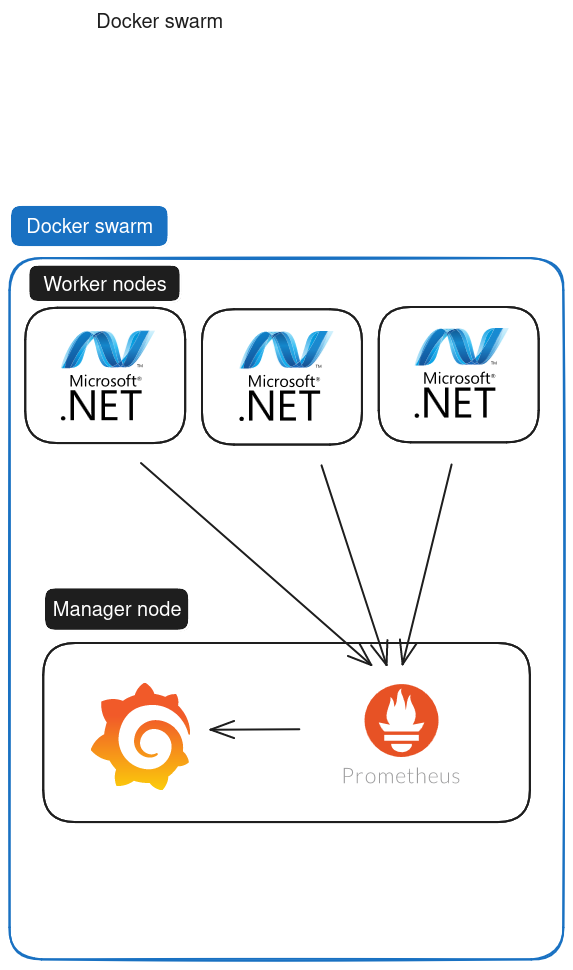
\includegraphics[width=1\textwidth]{Monitoring2.png}
	\caption{Diagram describing our monitoring implementation}
	\label{fig:Monitoring2}
\end{figure}
\begin{figure}[H]
	\centering
	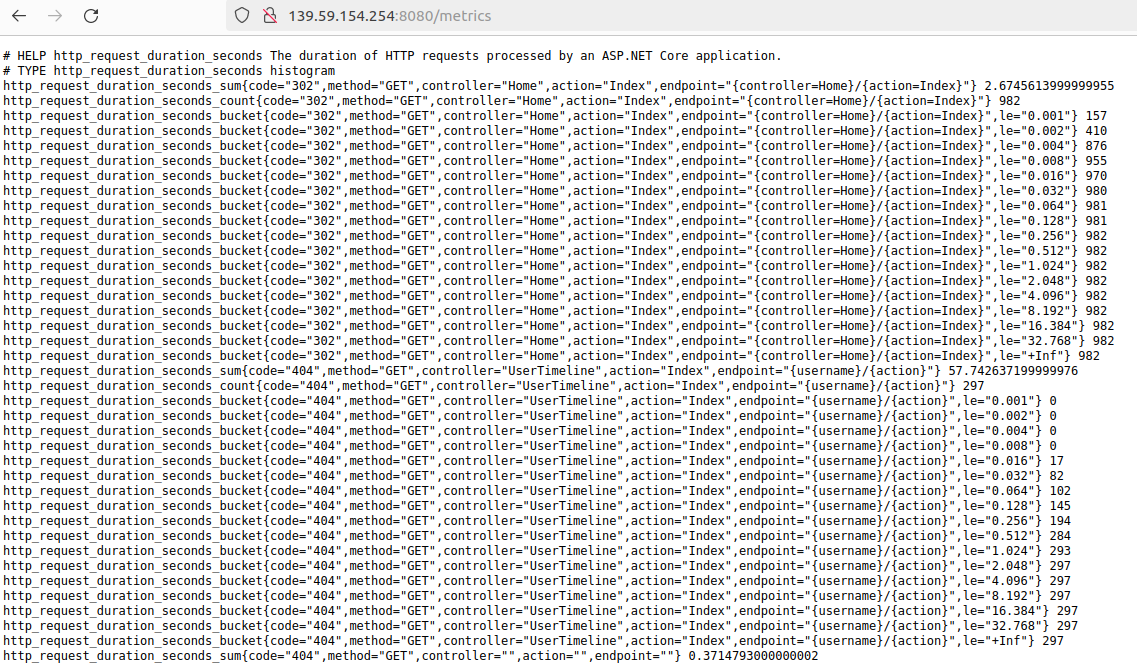
\includegraphics[width=1\textwidth]{metrics.png}
	\caption{Example of a worker nodes metrics page}
	\label{fig:metrics}
\end{figure}

\subsection{Monitoring configuration}
\paragraph{} Grafana and Prometheus are configured in a way, so that when initiating a docker swarm of with a manager nodes running docker images of them, then all necessary configuration gets set up automatically.

\subsubsection{Prometheus configuration}
\paragraph{} Prometheus gets configured using a yml file that gets inserted into the manager nodes Prometheus Docker image as a volume through a compose.yml file.

\subsubsection{Grafana configuration}
\paragraph{} Grafana data sources are set up using a .yml file that gets inserted into the manager into the manager nodes Grafana Docker image using volumes. The data source yml file contains variables about how to set up a Postgres database connection and a Prometheus monitoring connection.
\paragraph{} Additionally, two dashboards get added to the Grafana Docker image as json files. They contain all the variables and setup parameters required to automatically set up the required dashboards.
\paragraph{} Users are set up using a shell script. After the Grafana Docker image is running, a shell script sends a curl API call to the running Docker image every 5 seconds until success. The API call contains the users that are needed to set up automatically.